% !TEX root = ../FinalReport.tex
\chapter{User Acceptance Testing Report}

\section{Target Users Research}

\subsection{Target users}
This UAT invited a total of five bidder-side users from the transportation, energy,
and construction industries. Their positions include Tender Specialist, Project
Development, Sales Support, Business Development, and company CEO. The first four are
direct daily users of the system, while the CEO represents the manager who ultimately
decides whether the enterprise will participate in a given tender.

\subsection{Reasons for choosing these users}
These users are directly related to the core usage scenarios of GTM Agent and can
judge, from an actual business perspective:

\begin{enumerate}
\tightlist
\item whether the company recommended by the system is a reasonable potential bidder;
\item whether the matching score and explanation are credible enough;
\item whether the weight adjustment is in line with business judgment;
\item whether the operation process of the Agent is transparent and controllable.
\end{enumerate}

\subsection{Advantages and limitations of user research}
Testing with real industry personnel yields direct feedback with business context and
checks whether the product really solves the problem of bidding discovery and
potential-company screening. The participants' positions are diverse, including both
daily executives and decision-makers. The limitation is that the sample size is only
five people, so no general statistical inference can be made; participants' familiarity
with the bidding process also varies. Five participants are a common working minimum
for qualitative usability testing (Nielsen \& Landauer, 1993), but that argument
concerns the discovery of interface problems, not the estimation of population means:
the rating averages below are indications, not measurements. In addition, the test
uses system data and
scenarios prepared by the team, not the real private data of the participants'
enterprises.

\section{User Testing Design}

\subsection{Test method}
Each participant completes a structured think-aloud session (Ericsson \& Simon, 1993),
verbally expressing their judgments, confusions, and expectations while working, so
that reasoning is captured as it happens rather than reconstructed afterwards. The test
combines task scenarios with a
post-test questionnaire: first observing whether the user can complete the core
process, then collecting feedback through scale scoring and open-ended questions. The
UAT script is in Appendix A.

\subsection{Testing tasks}
Participants complete three core tasks in turn:

\begin{enumerate}
\tightlist
\item \textbf{Looking for candidate companies.} Choose a tender, check the companies
  recommended by the matcher, and judge whether the top-ranked company is a credible
  potential bidder.
\item \textbf{Adjust the matching weight.} Use the weight sliders to adjust factors
  such as semantic matching, budget, region, and qualification, and observe whether
  the ranking changes in real time as expected.
\item \textbf{Generate and review emails.} Generate an evidence-based outreach email
  for a candidate company, check whether it relates to the tender and company
  background, and judge whether it is usable after minor edits.
\end{enumerate}

\subsection{Evaluation indicators}
The test mainly evaluates: task completion, task time, lead quality (are the
recommended companies reasonable), explanation trust (does the user understand and
trust the ranking), email usability (usable after minor edits), agent trust and
transparency, overall usefulness / recommendation intention, and open feedback
(obstacles encountered and desired features). Scale items use 1--5 Likert points
(Likert, 1932), and the overall recommendation item uses the 0--10 Net Promoter
question (Reichheld, 2003).

\section{Analysis and Evaluation of Results}

\subsection{Main results}
The five participants rated overall usefulness at 4.1/5 in the post-test questionnaire
and willingness to recommend at 8.2/10; lead quality at 3.8/5, with email usability and
agent trust both at 3.7/5. Explanation trust had the lowest score, 3.4/5. Every
participant's recommendation intention was at least 7/10, indicating overall
recognition of the system's value. Scored as a Net Promoter Score (two promoters, three
passives, no detractors) the result is $+40$, although with five participants a single
detractor would move that by twenty points. All five reached the end of the core
workflow: two completed it fully and independently, while the other three needed minor
facilitator guidance and are recorded as partial completions. Time on task ranged from
18 to 28 minutes, with the fastest completions by the most frequent TED users.
Figures~\ref{fig:uat-participants} and~\ref{fig:uat-scores} report the per-participant
results and the resulting means.

\begin{figure}[!ht]
\centering
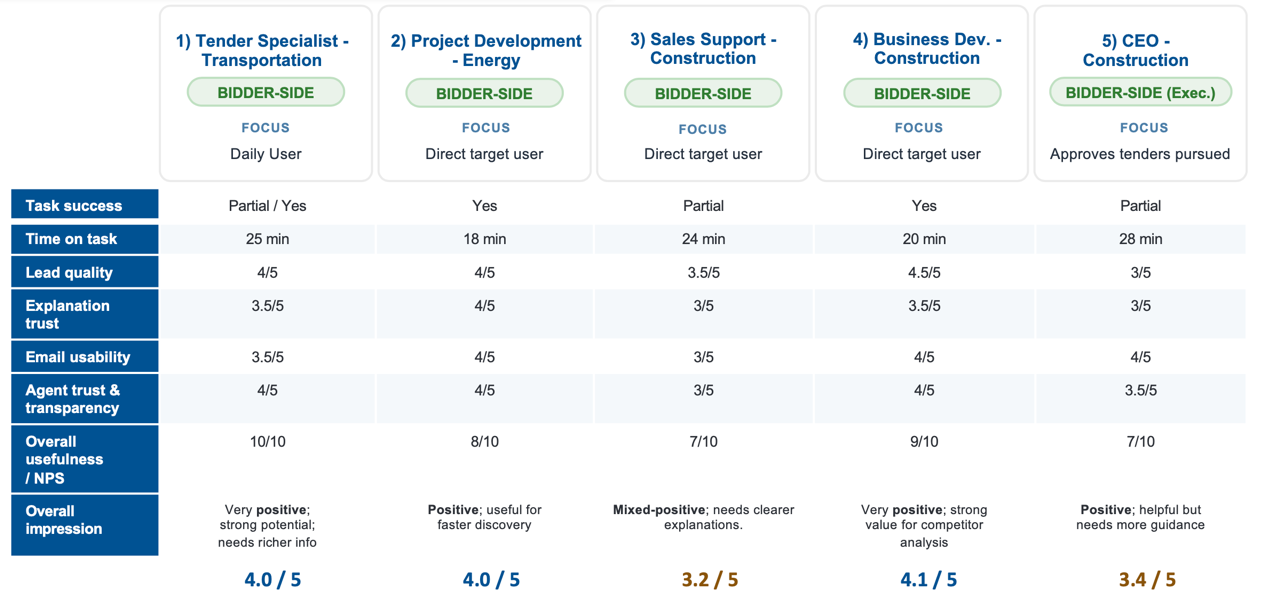
\includegraphics[width=0.78\linewidth]{uat_participants.png}
\caption[Per-participant UAT results]{Per-participant results; scale items use 1--5,
the recommendation item 0--10.\label{fig:uat-participants}}
\end{figure}

\begin{figure}[!ht]
\centering
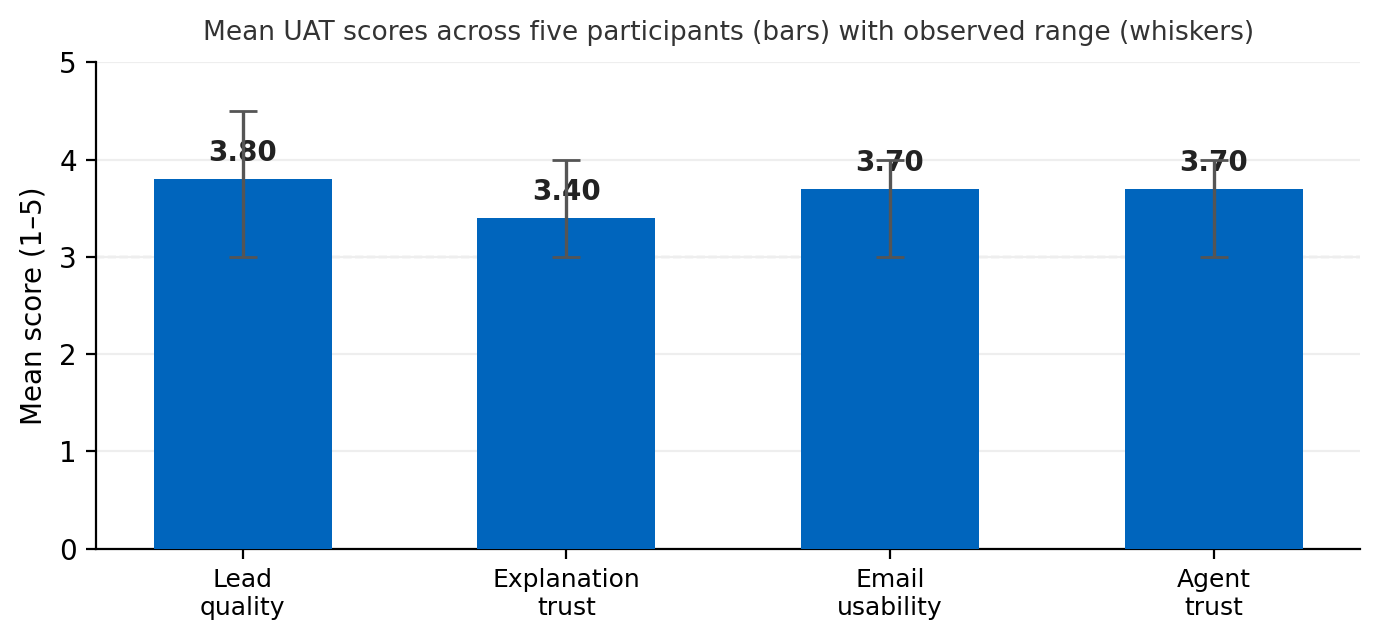
\includegraphics[width=0.55\linewidth]{uat_scores.png}
\caption[Mean UAT scores]{Mean UAT scores, whiskers showing the observed
range.\label{fig:uat-scores}}
\end{figure}

\subsection{Core findings}
Users generally believe the system reduces the time spent manually browsing TED and
searching for potential companies, and that the recommendations carry a certain
business rationality. However, users' understanding of ``why the ranking changes'' is
weak, so the natural-language explanation still needs strengthening --- reflected in the
lowest mean score, explanation trust (3.4/5). Participants could nonetheless read the
named ranking factors (semantic match, budget, region, qualification). All participants
also asked that the email directly present the tender's core information, such as
budget, deadline, and location.

\subsection{Feedback processing}
In response to concerns about insufficient email information, the team added a tender
summary block with budget, deadline, and location, removing the need to return to the
tender page before sending. The Agent Q\&A was also expanded so users can query tender,
company, and matching data, not just request recommendations. Requests that could not
be met within the MVP --- city fields, company-website links, shorter tender titles,
match alerts, and competitor analysis --- were recorded as future work.

\subsection{Conclusion}
UAT shows that GTM Agent does address the practical problems of target users in
discovering bidding opportunities, screening candidate companies, and preparing initial
outreach. Users most valued the efficiency gain and the lead quality, but trust in the
ranking explanation remains the most important area for improvement. Subsequent
development should therefore prioritise the natural-language explanation, supplement
key tender and company information, and retain human review of emails and results.
